% !TEX root = ../main.tex
\begin{titlepage}
\thispagestyle{empty}
\begin{center}
    % --- Official Logo ---
    \vspace*{-1cm}
    
\includegraphics[width=8cm]{logos/LA_SALLE-1000x340.jpg}\\[1.2cm]
    
    % --- Faculty and Degree ---
    {\large \textbf{Facultat Internacional de Comerç i Economia Digital La Salle}}\\[0.4cm]
    {\Large \textbf{Treball de Final de Màster}}\\[0.3cm]
    {\large Màster Universitari en Ciència de les Dades / Data Science}\\[1.8cm]
    
    % --- Title Box ---
    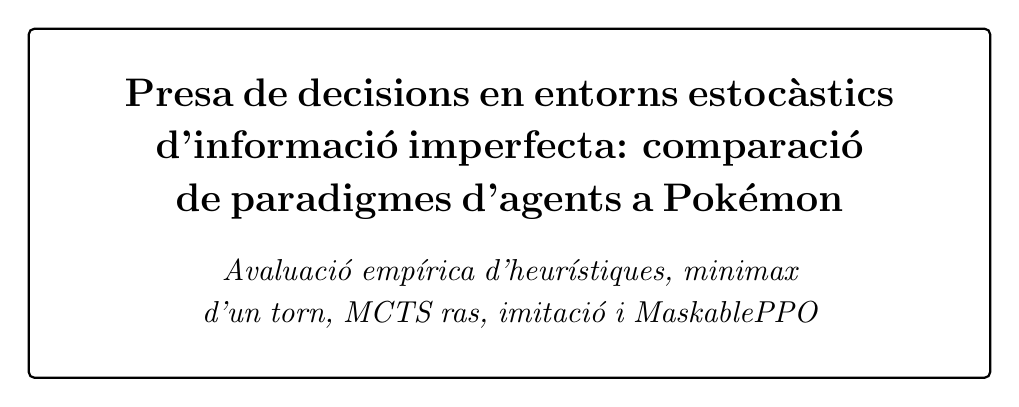
\begin{tikzpicture}
        \node[draw=black, line width=0.8pt, rounded corners=2pt, inner xsep=15pt, inner ysep=18pt, text width=0.92\textwidth, align=center] {
            {\fontsize{14pt}{19pt}\selectfont\bfseries Presa de decisions en entorns estocàstics d'informació imperfecta: comparació de paradigmes d'agents a Pokémon\par}
            \vspace{0.35cm}
            {\fontsize{11pt}{15pt}\selectfont\itshape Avaluació empírica d'heurístiques, minimax d'un torn, MCTS ras, imitació i MaskablePPO\par}
        };
    \end{tikzpicture}
    
    \vfill
    
    % --- Candidate and Supervisor Details ---
    \begin{tabularx}{\textwidth}{@{}X r@{}}
        \textbf{Alumne/a:} & \textbf{Professor/a Ponent:} \\[1ex]
        Gerard Pascual Fontanilles & Jordi Peralta Dolz
    \end{tabularx}\\[1.5cm]
    
    % --- Date & Location ---
    {\small Barcelona, Agost 2026}
\end{center}
\end{titlepage}

% --- Acta d'avaluació del Tribunal ---
\clearpage
\thispagestyle{empty}
\begin{center}
    \vspace*{0.5cm}
    {\Large \textbf{ACTA D'EXAMEN DEL TREBALL DE FINAL DE MÀSTER}}\\[1.5cm]
\end{center}

\noindent
Reunit el Tribunal qualificador en el dia de la data, l'alumne/a:\\[1.5ex]
\textbf{Gerard Pascual Fontanilles}\\[2.5ex]
Va exposar el seu Treball de Final de Màster, el qual va tractar sobre el tema següent:\\[1.5ex]
\textbf{Presa de decisions en entorns estocàstics d'informació imperfecta: comparació de paradigmes d'agents a Pokémon}\\[2.5ex]
Acabada l'exposició i contestades per part de l'alumne/a les objeccions formulades pels membres del tribunal, aquest va valorar l'esmentat Treball amb la qualificació de:\\[3ex]

\begin{center}
    \setlength{\tabcolsep}{24pt}
    \renewcommand{\arraystretch}{2.2}
    \begin{tabular}{|c|c|}
        \hline
        \textbf{Qualificació Qualitativa} & \textbf{Qualificació Numèrica} \\
        \hline
        \rule{0pt}{35pt} & \\
        \hline
    \end{tabular}
\end{center}

\vspace{1.8cm}
\noindent
Barcelona, a \rule{1.2cm}{0.4pt} de \rule{3.5cm}{0.4pt} de 2026\\[3.0cm]

\noindent
\begin{minipage}[t]{0.45\textwidth}
    \centering
    \rule{5.5cm}{0.4pt}\\[0.5ex]
    \textbf{VOCAL DEL TRIBUNAL}
\end{minipage}\hfill
\begin{minipage}[t]{0.45\textwidth}
    \centering
    \rule{5.5cm}{0.4pt}\\[0.5ex]
    \textbf{VOCAL DEL TRIBUNAL}
\end{minipage}

\vspace{2.5cm}
\begin{center}
    \rule{6cm}{0.4pt}\\[0.5ex]
    \textbf{PRESIDENT DEL TRIBUNAL}
\end{center}

\clearpage
